\documentclass[a4paper]{article}
\usepackage[latin1]{inputenc}
\usepackage{hyperref}
\usepackage{verbatim}
\newcommand{\daisy}{Daisy}
\newcommand{\Daisy}{Daisy}
\newcommand{\cplusplus}%
{{\leavevmode{\rm{\hbox{C\hskip -0.1ex\raise 0.5ex\hbox{\tiny ++}}}}}}
\newcommand{\Cplusplus}{\cplusplus}
\newcommand{\mshe}{Mike/\textsc{she}}
\newcommand{\wintel}{\texttt{win32}}
\newcommand{\dll}{\textsc{dll}}
\newcommand{\Dll}{\textsc{Dll}}
\newcommand{\gui}{\textsc{gui}}
\newcommand{\Gui}{\textsc{Gui}}
\newcommand{\unix}{Unix}
\newcommand{\dhi}{\textsc{dhi}}
\newcommand{\Dhi}{\textsc{Dhi}}
\newcommand{\api}{\textsc{api}}
\newcommand{\Api}{\textsc{Api}}
\newcommand{\lai}{\textsc{lai}}
\newcommand{\Lai}{\textsc{Lai}}
%\newcommand{\url}[1]{\linebreak[4]\texttt{<URL:#1>}}

%%% Local Variables: 
%%% mode: latex
%%% TeX-master: t
%%% End: 

\bibliographystyle{apalike}
\usepackage{graphicx}

\begin{document}

\title{\textbf{Initializing organic matter pools}}
\author{
    Per Abrahamsen, S�ren Hansen and Henrik Svendsen\\
    The Royal Veterinary and Agricultural University\\
    Department of Agricultural Sciences\\
    Laboratory for Agrohydrology and Bioclimatology
}
\date{\today}
\maketitle

\begin{abstract}
  Organic matter models using multiple pools for soil biomass and soil
  organic matter have proved able to simulate both short term and long
  term change in humus content of agricultural soil.  However, these
  pools do not correspond to measurable physical quantities, and are
  therefore difficult for a non-expert to understand and use, and
  fragile with respect to changes in the model.  An alternative
  sometimes used is to assume the organic matter is in a state of
  equilibrium.  Unfortunately, the time to reach equilibrium is often
  measured in centuries, so this assumptions is unlikely to hold true.
  For the same reason, the use of a warmup period cannot replace the
  need for a good initial partitioning.  In this paper we propose a
  milder assumption, namely a quasi-equilibrium where all but the
  slowest pool is in equilibrium with the amount of carbon input.
  This assumption allows the non-expert user to initialize the model,
  and is robust with regard to model changes.
\end{abstract}

\tableofcontents
\pagebreak

\section{Soil organic matter modelling}

SH: referencer til vigtigste org.matter modeller.

It is conventional to divide the organic matter in the soil into three
fractions.  First we have the freshly entered organic matter, which
can still be traced back to its origin.  For a cultivated soil, this
might include organic fertilizer, crop residuals, including
rhizodeposition and dead leaves incorporated to the soil by
earthworms.  This fraction is conventionally called \emph{added
  organic matter}, or \textsc{aom}.  Then we have the \emph{soil
  microbial biomass}, or \textsc(smb), the living part of the organic
matter, excluding roots.  Finally we have the humus, the \emph{soil
  organic matter} (\textsc{som}), which can no longer be traced back
to its origin.  The dynamics of the system consist of input in the
form of new added organic matter, and turnover in the form the soil
biomass eating the other matter (and itself).

In numeric models, these fractions may be further divided into smaller
pools, the content of each pool assumed by the model to have uniform
properties, e.g.\ similar turnover rate and C/N ratio.  Having two
\textsc{som} and two \textsc{smb} pools allows a well calibrated model
to capture both the short term (see XXX) and long term (XXX) dynamics
of the system.  If you are only interested in accuracy on a single
time scale, less pools may be needed.  The number of \textsc{aom}
pools needed also depends on what you are simulating.  For batch
experiments and some long time scenarios, a single pool may be enough.
To simulate input sources from real farming, two pools per source are
in general needed per source.

In several comparisons (see XXX, YYY, ZZZ), \daisy{} (see XYZZY) has
been among the best models for both short and long term predictions of
soil matter, and \daisy{} will be the reference for the rest of this
article.  Apart from soil organic matter, \daisy{} also simulate a
number of other processes, such as water, heat and nitrogen dynamics
in the soil, as well as biocliamte, crop development and management.

\section{Evolution of the Daisy model}

The purpose of the \daisy{} model is to simulate real farming
practice, both on the short and the long term.  Thus, we get a system
with two pools for each of \textsc{som} and \textsc{smb}, and two
pools for each type of fertilizer applied and crop residual left on the
field.  The original model is depicted in figure~\ref{fig:om1}.
\begin{figure}[htbp]
  \centering
  
  \caption{The original Daisy OM parameterization.}
  \label{fig:om1}
\end{figure}

PA: turnover rates, fractions, efficiency, maintenance, (abiotic factors).

The \daisy{} software allows the user to adjust all of these
parameters.  It also allows the user to specify the number of \textsc{som}
and \textsc{smb} pools, as well as the number of \textsc{aom} pools for each
fertilizer application and each crop residual type.  It thus provides
a good basis for experimentation.

The first such experimental change that made it back into \daisy{} was
made by Torsten M�ller (see XXX 19??), who adjusted the turnover rates
of the \textsc{smb} pools so the biomass content of the soil better
matched the levels measured at the fields.  The change did not affect
the long time dynamics of the systen.  The second such change was made
by Anders Sanders (see XXX 19??).  The was a complete recalibration
that took into account the carbon input from rhizodepositions.  This
change was more radical, involving both turnover rates and directions
of flow, and made the system much more adaptable to new levels of
input, another effect which has also been observed emperically (see
DJF repport on humus levels).

The current model is depicted in~\ref{fig:om2}.  The purpose of the
SOM3 pool in that figure will be explained later.
\begin{figure}[htbp]
  \centering
  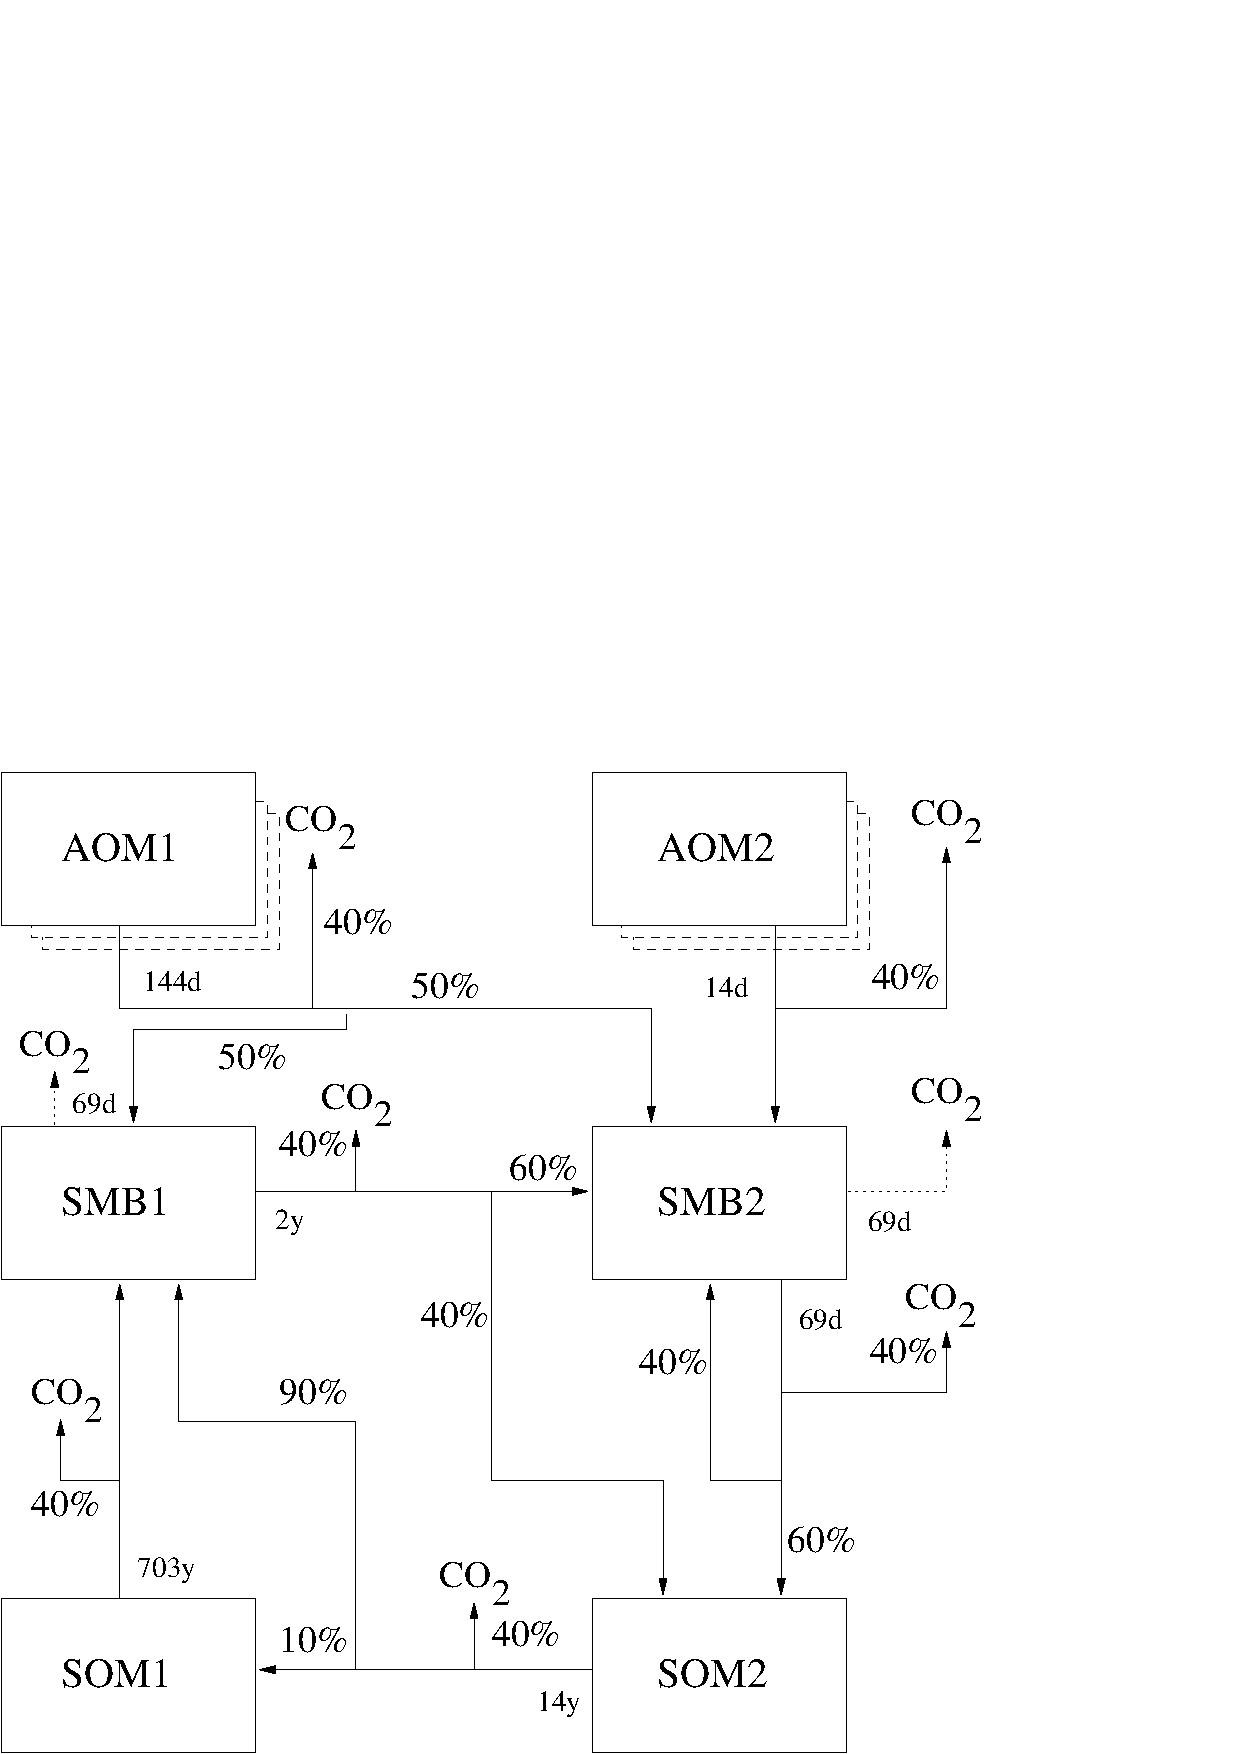
\includegraphics[width=0.8\hsize]{om1}
  
  \caption{New parameterization.}
  \label{fig:om2}
\end{figure}

Some of the experimental changes affecting soil organic matter that we
are currently working on, and which may be included in future versions
of \daisy{}, are dissolved organic matter (see BGJ), another
recalibration based on a larger experimental database and with special
focus on the effect of clay (see Biomod/Bj�rn/AP), and some wishlist
items includes phosphor dynamics and a calibration for forrest soil.
The conclusion is that model has changed in the past, and will
continue to change in the future.

\section{Expanding user base}

The original development of \daisy{} was founded by the Danish
environmental protection agency \cite{daisy-def}, and the first
non-research use was made by expert users who evaluated the national
environmental plans for limiting nitrogen contamination of groundwater
and surface water (see VMPuse).  Since then, \daisy{} has been used in
other parts of the environmental and agricultural agencies (see
NORVANA XXX), as well as increasingly by local authorities for
evaluating regional plans (see �rhus Amt og XXX), and recently also
for evaluation of applications for changed farm practice at an
individual farm level (see VVM, PLANTINFO).  For the last case,
\daisy{} has also been used by consulting agencies representing ``the
other side'', namely farmers seeking permission to change farming
practice.

The effect of this increased use has been that we no longer can rely
on the users being experts.  Therefore, a project was started in order
to provide standardized procedures for setting \daisy{} simulations
(see XXX).  As part of this project, most components of \daisy{} was
evaluated in order to find parameters and submodels who could be
initialized automatically from default values, or from other
parameters.  These parameters and submodels are still available to the
expert user, but will be hidden for the user who do not have the
expertice or data available.  The result is that the software now
appears much simpler to the user, even though no substantial changes
to the model have been made.

The partition of the organic matter into the various soil pools have
been a particular stumbling block for most users, partly because it
does not reflect an easily identificable property of the system being
modellen.  

\section{The equilibrium assumption}

It is common to use an equilibrium assumption for initialising models
where measurements are not available.  For example, in \daisy{} we
assume that the soil water in the bottom of the unsaturated zone is in
equilibrium with the groundwater, as specified by Darcy's equation.
There are two reasons equilibrium is often a good assumption.  For
some systems, it will be correct most of the time, because they quicly
reach equilibrium compared to the externaly imposed changes.  In other
cases, the dynamic of the system quickly dominate over the initial
condition, so an equilibrium is good for giving a reasonable initial
state.

As part of Sander's recalibration work, he also found that the ratio
between the \textsc{som1} and \textsc{som2} for a system in equilibrium will
49\% vs 51\%.  Since \daisy{} after his recalibration required users
to readjust the partitioning between \textsc{som1} and \textsc{som2}, there
was a strong tendency that users just picked the equilibrium values.

\section{Long term simulations}

As part of the standardization project mentioned earlier (see XXX),
Henrik Svendsen used \daisy{} to simulate the effect on soil organic
matter of changing farming practice.  Figure~\ref{fig:clayom} shows a
system that goes from equilibrium at a high level of carbon input, to
equilibirum at a low level of carbon input.  Danish farming practice
has been used, as well as Danish climate and soil.  The soil has a for
Danish conditions high clay content (10\%).
Figure~\ref{fig:clayratio} shows the \textsc{som1}/\textsc{som2}
ratio, which is can be used for initializing \daisy{}.  Finally,
figure~\ref{fig:sandratio} shows the ration for simulation on a coarse
sandy soil going from a low to high input equilibrium.
\begin{figure}[htbp]
  \centering

  \caption{Long term simulation of organic matter content from
    changing from high to low input on a clayish loam.}
  \label{fig:clayom}
\end{figure}
\begin{figure}[htbp]
  \centering

  \caption{Long term simulation of \textsc{som1}/\textsc{som2} ratio
    from changing from high to low input on a clayish loam.}
  \label{fig:clayratio}
\end{figure}
\begin{figure}[htbp]
  \centering
  
  \caption{Long term simulation of \textsc{som1}/\textsc{som2} ratio
    from changing from low to high input on a coarse sandy soil.}
  \label{fig:sandratio}
\end{figure}

As can be seen, the time to reach a new equilibirum after a change in
farming practice can be several centuries, which makes it safe to
assume that no Danish farming land is in equilibrium.  At such a time
scale, not only farming practice but also climate is going to change.

As a conclusion, we need a way to initialize the soil organic matter
that is robust with regard to changes in the model or model
parameterization, and at the same time expressible in terms of
physical properties the user can understand.  And we cannot use the
most obvious initialization condition, namely an equilibrium
assumption.

\section{Equations}

In order to find a better way to initialize the organic matter pools,
we will start by looking at their internal relationships.
\begin{eqnarray}
  \Delta\mbox{\textsc{smb1}} &=& a\> \mbox{\textsc{smb1}} + b\>
  \mbox{\textsc{smb2}} + c\> \mbox{\textsc{som1}} + d\>
  \mbox{\textsc{som2}} + e\, \Delta\mbox{\textsc{aom}}\\
  \Delta\mbox{\textsc{smb2}} &=& f\> \mbox{\textsc{smb1}} + g\>
  \mbox{\textsc{smb2}} + h\> \mbox{\textsc{som1}} + i\>
  \mbox{\textsc{som2}} + j\, \Delta\mbox{\textsc{aom}}\\
  \Delta\mbox{\textsc{som1}} &=& k\> \mbox{\textsc{smb1}} + l\>
  \mbox{\textsc{smb2}} + m\> \mbox{\textsc{som1}} + n\>
  \mbox{\textsc{som2}} + o\, \Delta\mbox{\textsc{aom}}\\
  \Delta\mbox{\textsc{som2}} &=& p\> \mbox{\textsc{smb1}} + q\>
  \mbox{\textsc{smb2}} + r\> \mbox{\textsc{som1}} + s\>
  \mbox{\textsc{som2}} + t\, \Delta\mbox{\textsc{aom}}
\end{eqnarray}
Here, we have excluded the \textsc{aom} pools, except as a source for
the other pools which we denote $\Delta\mbox{\textsc{aom}}$.
$\Delta\mbox{\textsc{aom}}$ is the total carbon input to the system.
The \textsc{aom} pools are special in that they are not feed by any of
the other pools, but by outside sources such as crop residuals and
fertilizer.  The other pools are described by content (\textsc{smb1},
\textsc{smb2}, \textsc{som1}, or \textsc{som2}) and change of content
($\Delta\mbox{\textsc{smb1}}$, $\Delta\mbox{\textsc{smb2}}$,
$\Delta\mbox{\textsc{som1}}$, $\Delta\mbox{\textsc{som2}}$).

The factors $a$ to $t$ depend on the model, so the factors are
different for the original model (figure~\ref{fig:om1}) and the Sander
recalibration (figure~\ref{fig:om2}).  They also depend on site and
time specific factors, namely the clay content of the soil, the
temperature, and the water potential.

Some of these factors may be zero, in none of the calibrations
mentioned we have any carbon going directly from the \textsc{aom}
pools to \textsc{som1}, so $o$ will always be zero.  The reason we
include these, is that we are trying to solve the initialization
problem in a way that is robust with regard to changes in the model.
The description is also robust with regard to the number of
pools\footnote{The generalized form is: 
  \begin{displaymath}
    \begin{array}{rclcr}
      \Delta\mbox{\textsc{smb}}i &=& \displaystyle
      \sum_{k=1}^{\mbox{\tiny\#\textsc{smb}}} a_{i,k}\,\mbox{\textsc{smb}}k + 
      \sum_{l=1}^{\mbox{\tiny\#\textsc{som}}} b_{i,l}\,\mbox{\textsc{som}}l +
      c_i \Delta\mbox{\textsc{aom}} 
      &;&i = 1\ldots\mbox{\#\textsc{smb}}\nonumber\\
      \Delta\mbox{\textsc{som}}j &=& \displaystyle
      \sum_{k=1}^{\mbox{\tiny\#\textsc{smb}}} d_{j,k}\,\mbox{\textsc{smb}}k +
      \sum_{l=1}^{\mbox{\tiny\#\textsc{som}}} e_{j,l}\,\mbox{\textsc{som}}l +
      f_j \Delta\mbox{\textsc{aom}} 
      &;&j = 1\ldots\mbox{\#\textsc{som}}\nonumber
    \end{array}
  \end{displaymath}
}, adding a new pool will just one more equation, and two new unknowns.

Back to the two pool example.  We have four equations and nine
unknowns.  We need more information.  The first piece of information
we can add is the total organic matter content in the field, which can
be directly measured.  This give is one new equation, and two new
variables.
\begin{equation}
  \label{eq:total}
  \mbox{\textsc{total}} = \mbox{\textsc{smb1}} + \mbox{\textsc{smb2}}
  + \mbox{\textsc{som1}} + \mbox{\textsc{som2}} + \mbox{\textsc{aom}}
\end{equation}
\textsc{total} is measured.  \mbox{\textsc{aom}}, the initial content
of added organic matter, is given a default value corresponding to
typical root residuals left from a crop.  We now miss four equations,
one for each pool.

The equilibrium assumption corresponds to adding these four equations: 
\begin{displaymath}
  \Delta\mbox{\textsc{smb1}} = \Delta\mbox{\textsc{smb2}} 
  = \Delta\mbox{\textsc{som1}} = \Delta\mbox{\textsc{som2}} = 0
\end{displaymath}
Even though we earlier argued that it was not good for initializing
the system, we can use it to obtain an estimate of
$\Delta\mbox{\textsc{aom}}$, the carbon input level required to
maintain the measured amount of organic matter in the soil.

The initializing procedude we ended up using was to allow the slowest
pool (which happens to be \textsc{som1}) to change, but require the
user specify the carbon input to the system ($u$).  We then get:
\begin{eqnarray}
  \Delta\mbox{\textsc{smb1}} &=& 0\\
  \Delta\mbox{\textsc{smb2}} &=& 0\\
  \Delta\mbox{\textsc{som2}} &=& 0\\\label{eq:fastpooleq}
  \Delta\mbox{\textsc{aom}} &=& u
\end{eqnarray}

We now have nine equations with nine unknowns, and can initialize the
system.  The physical interpretation of this initialization is that
all but the slowest pool has reach a quasi-equilibrium with respect to
the input, and the size of the slowest pool.  Since the slowest pool
is still changing (and the other pools will have to change to reflect
that), this is not a true equilibrium.

We also have a model independent knob for users who want to calibrate
the system.  If the user can estimate the total rate of change in
carbon content, i.e.\ is the soil gaining or losing organic matter
with the specified input, we can substitute
equation~\ref{eq:fastpooleq} with
\begin{displaymath}
  \Delta\mbox{\textsc{smb1}} + \Delta\mbox{\textsc{smb2}} 
  + \Delta\mbox{\textsc{som1}} + \Delta\mbox{\textsc{som2}} = v
\end{displaymath}
where $v$ is the user specified change in carbon content.  Since out
users are generally more concerned with nitrogen than with carbon, we
ask them to specify the \emph{background mineralization} ($w$), which
is the amount of nitrogen the rest of the system gets or loses from
the soil.  The equation is then
\begin{displaymath}
  \frac{\Delta\mbox{\textsc{smb1}}}{{C/N}_{\mbox{\small\textsc{smb1}}}}
  + \frac{\Delta\mbox{\textsc{smb2}}}{{C/N}_{\mbox{\small\textsc{smb2}}}}
  + \frac{\Delta\mbox{\textsc{som1}}}{{C/N}_{\mbox{\small\textsc{som1}}}}
  + \frac{\Delta\mbox{\textsc{som2}}}{{C/N}_{\mbox{\small\textsc{som2}}}}
  = w
\end{displaymath}
The simulated background mineralization will only be the specified
value ($w$) if the simlated carbon input also corresponds to the
specified value ($u$).

In conclusion, we can now initialize the soil organic matter system
from two or three numbers supplied by the user.  The two mandatory
numbers are the total content of organic matter, and an estimate of
how much carbon has been added to the system per year in the recent
decades.  The third, optional, number is the estimated background
mineralization.  The first number is directly measurable, the two
other can at least be understood by people who have no intimate
knowledge of the model, and can be estimated by the user from \daisy{}
simulations.  None of the numbers will have to be changed when the
model itself is changed.

\section{Assumptions and limitations}

In the equations we used a large number of constants, without
indicating how we calculate them.  Here is the formula for calculating
$a$ from the first equation.
\begin{displaymath}
  a = t_{\mbox{\tiny\textsc{smb1}}}\,
  (X_{\mbox{\tiny\textsc{smb1}}\rightarrow{\mbox{\tiny\textsc{smb1}}}}\,
  E_{\mbox{\tiny\textsc{smb1}}\rightarrow{\mbox{\tiny\textsc{smb1}}}}
  - 1) - m_{\mbox{\tiny\textsc{smb1}}})\,
  F_{\mbox{\tiny\textsc{smb1}}}^T (T)\,
  F_{\mbox{\tiny\textsc{smb1}}}^\psi (\psi)\,
  F_{\mbox{\tiny\textsc{smb1}}}^C (X_c)
\end{displaymath}


-- clay, T og h

T=10 dg

-- top horizons.

\section{Results}

Validation.  Lange tidsserier af Per og S�ren.

FIG: SOM1/SOM2 ratio (sim + eq)  after change in management high->low, clay
FIG: SOM1/SOM2 ratio (sim + eq)  after change in management low->high,
sand

lim 70\%

Brug i standardisering.

\section{Bibliography}
\bibliography{daisy}

\end{document}

%%% Local Variables: 
%%% mode: latex
%%% TeX-master: t
%%% End: 
